\documentclass[10pt,twocolumn]{article}

\usepackage[a4paper,margin=0.72in]{geometry}
\usepackage{mathptmx}
\usepackage{microtype}
\usepackage{booktabs}
\usepackage{tabularx}
\usepackage{array}
\usepackage{enumitem}
\usepackage{graphicx}
\usepackage{xurl}
\usepackage[hidelinks]{hyperref}
\usepackage{titlesec}
\usepackage{tikz}
\usetikzlibrary{arrows.meta,positioning,fit,shapes.geometric}

\titleformat{\section}{\large\bfseries}{\thesection}{0.5em}{}
\titleformat{\subsection}{\normalsize\bfseries}{\thesubsection}{0.5em}{}
\setlist[itemize]{leftmargin=*,nosep}
\setlength{\parindent}{0.9em}
\setlength{\parskip}{0pt}
\renewcommand{\arraystretch}{1.15}

\title{\vspace{-1.5em}\bfseries Organoid Brain-on-a-Chip Systems: Resource Map, Bioelectronic Interface Strategy and First-Demo Roadmap}
\author{\begin{tabular}{c}Lachlan Chen \quad AgintiFlow\\Aginti Lab, LazyingArt LLC\end{tabular}}
\date{Curated 31 May 2026}

\begin{document}
\maketitle

\begin{abstract}
\noindent Brain-on-a-chip research is converging with human brain organoids, microfluidics, multielectrode arrays (MEAs), soft bioelectronics and biological computing. This survey maps high-value resources and turns them into a buildable roadmap. The key engineering thesis is simple: biology connects to electronics through a stable extracellular interface, not through direct digital access to cells. A feasible first demo should therefore avoid wet-lab complexity and prove the loop in software first: spike-like data, preprocessing, burst/network features, a decoder or reservoir readout, a stimulation policy, and a safety gate. Wet biology can then be added through a remote platform or commercial MEA before attempting custom 3D organoid chips.
\end{abstract}

\textbf{Keywords:} brain organoid; brain-on-chip; organoid intelligence; wetware computing; microelectrode array; microfluidics.

\section{Scope}

This document treats ``brain on a chip with organoids'' as four overlapping systems: brain organoids maintained in engineered devices, brain organoids interfaced to MEAs or soft electrodes, closed-loop biological computing platforms, and software/data resources for analysing organoid activity. It is a high-confidence research map, not a claim that every marginal paper in the broader organoid literature has been enumerated.

\section{Landscape}

Three technical bottlenecks dominate. First, organoids need vascular, metabolic, immune and extracellular-matrix support to mature reproducibly. Microfluidics helps by adding flow, oxygenation, gradients and repeatable dosing. Second, planar MEAs undersample spherical tissues. New devices therefore wrap, embed, suspend or penetrate organoids using shells, meshes, liquid metals and multilayer electrodes. Third, organoid computing requires closed-loop stimulation, stable readout, shared data formats and defensible interpretation of learning-like behaviour.

\section{Core Literature}

\begin{table*}[t]
\small
\caption{Curated papers and reviews that anchor the organoid brain-on-chip topic.}
\begin{tabularx}{\textwidth}{p{0.17\textwidth}p{0.28\textwidth}X}
\toprule
\textbf{Theme} & \textbf{Resource} & \textbf{Why it matters} \\
\midrule
Foundation & Lancaster et al., cerebral organoids, 2013 \cite{lancaster2013} & Establishes self-organized cerebral organoids as human brain development models. \\
On-chip folding & Karzbrun et al., human brain organoids on a chip, 2018 \cite{karzbrun2018} & Uses chip-constrained organoids to study mechanics of cortical folding. \\
Toxicology chip & Wang et al., prenatal nicotine exposure, 2018 \cite{wang2018} & Early hiPSC brain organoid-on-chip disease/toxicology platform. \\
Microfluidic assembly & Ao et al., prenatal cannabis exposure, 2020 \cite{ao2020} & One-stop microfluidic brain organoid assembly and exposure model. \\
Maturation & Cho et al., brain ECM plus microfluidic flow, 2021 \cite{cho2021} & Shows brain ECM and dynamic microfluidics improve survival, maturation and electrophysiology. \\
Neuroinflammation & Ao et al., immune-competent/tubular organoids, 2021 \cite{ao2021} & Adds microfluidic culture strategies for inflammatory modelling. \\
Preclinical review & Castiglione et al., 2022 \cite{castiglione2022} & Focused review of human brain organoids-on-chip for preclinical use. \\
Disease review & Zhang et al., 2025 \cite{zhang2025} & Recent review of history, challenges and neural disease modelling trends. \\
Integration review & Zhao et al., 2024 \cite{zhao2024} & Broad Nature Reviews map of organoid--organ-on-chip integration. \\
\midrule
MEA pipeline & MEA-NAP paper, 2024 \cite{meanap2024} & Practical network analysis pipeline for 2D cultures and 3D brain organoids. \\
HD-MEA readout & Functional imaging using high-density MEAs, 2022 \cite{hdmea2022} & Demonstrates single-unit and network measurements in human cerebral organoids. \\
3D MMF & Park et al., 3D multifunctional neural interfaces, 2021 \cite{park2021} & Flexible 3D devices for cortical spheroids and engineered assembloids. \\
Cyborg organoids & Li et al., 2019; Le Floch et al., 2022 \cite{li2019,lefloch2022} & Mesh nanoelectronics integrated through organogenesis for chronic tissue-wide recordings. \\
Shell MEA & Huang et al., 2022 \cite{huang2022} & Self-folding shell electrodes encapsulate brain organoids for 3D surface readout. \\
Liquid-metal interface & Wu et al., 2024 \cite{wu2024} & Stretchable 128-channel liquid-metal mesh interface for hippocampal organoids. \\
Reshapable MEA & Magnetically reshapable liquid-metal 3D MEAs, 2025 \cite{magnetic2025} & Adjustable soft 3D electrodes for intra-organoid electrophysiology. \\
Depth MEA & Kim et al., multilayered MEA, 2026 \cite{kim2026} & Depth-resolved multilayer recordings across cerebral organoid vertical structure. \\
Full-coverage interface & Liu et al., shape-conformal porous frameworks, 2026 \cite{shapeconformal2026} & Nearly full surface coverage, high-channel-count electrophysiology and programmed stimulation for neural organoids. \\
\midrule
Organoid intelligence & Smirnova et al., OI, 2023 \cite{smirnova2023} & Defines organoid intelligence as a field combining brain organoids and machine interfaces. \\
Ethics roadmap & Baltimore Declaration and OI workshop, 2023 \cite{baltimore2023,workshop2023} & Establishes governance and community framing for OI. \\
Brainoware & Cai et al., 2023 \cite{cai2023} & Brain organoid reservoir computing for speech recognition and nonlinear prediction. \\
DishBrain & Kagan et al., 2022 \cite{kagan2022} & Closed-loop cultured-neuron system embodied in a Pong-like environment. \\
Sample efficiency & Khajehnejad et al., 2024 \cite{khajehnejad2024} & Compares biological neural cultures with deep RL agents in a simulated game. \\
Remote platform & FinalSpark Neuroplatform paper, 2024 \cite{finalspark2024} & Remote API/Jupyter access to living neuronal/organoid electrophysiology. \\
Computing overview & Talavera and Ulmann, 2025 \cite{talavera2025} & Broad overview of brain organoid computing and bibliography. \\
Tactile encoding & Liu et al., 2025/2026 \cite{liu2025} & Braille-like tactile classification using stimulated forebrain organoids. \\
\bottomrule
\end{tabularx}
\end{table*}

\section{Repositories}

\begin{table*}[t]
\small
\caption{Code and data repositories worth tracking or vendoring as references.}
\begin{tabularx}{\textwidth}{p{0.23\textwidth}p{0.18\textwidth}X}
\toprule
\textbf{Repository} & \textbf{Type} & \textbf{Use} \\
\midrule
\url{github.com/SAND-Lab/MEA-NAP} & MEA analysis & Network topology, burst, connectivity and batch analysis for MEA recordings. \\
\url{github.com/Cortical-Labs/cl-api-doc} & Platform docs & Early CL1 API notebooks for closed-loop neuron experiments. \\
\url{github.com/Cortical-Labs/cl-sdk} & SDK/simulator & Python simulator for Cortical Labs API workflows. \\
\url{github.com/Cortical-Labs/SpikeStream} & Visualization & Real-time spike-stream visualization code. \\
\url{github.com/TBC-TJU/MetaBCI} & BCI software & Open-source BCI algorithms and stimulation/brainflow tooling already vendored locally. \\
\url{github.com/quadbio/primate_cerebral_organoids} & Reproducibility & Code for primate cerebral organoid single-cell analyses. \\
\url{github.com/quadbio/organoid_regulomes} & Reproducibility & Cell-fate regulome analysis in human cerebral organoids. \\
\url{github.com/utokyoIkeuchilab/neural-organoid-activity-MEA-analysis} & MEA analysis & Activity analysis for connected cerebral organoids. \\
\url{github.com/danielathome19/pyorganoid} & Simulation & Python package for organoid intelligence and organoid learning simulation. \\
\url{github.com/McD-NMI/OrganoidMEA} & Simulation/analysis & Electrophysiology simulation and analysis for OrganoidMEA. \\
\url{github.com/Unlimited-Research-Cooperative/human-cortical-organoid-intelligence-system} & Concept/demo & Human cortical organoid intelligence system experiments and notes. \\
\url{github.com/aimarket/awesome-autonomous-drone-racing} & Robotics reference & Locally vendored robotics/RL reference; useful only for downstream closed-loop embodied tasks. \\
\bottomrule
\end{tabularx}
\end{table*}

\section{Projects and Platforms}

\begin{table*}[t]
\small
\caption{Active projects, companies, platforms and programs.}
\begin{tabularx}{\textwidth}{p{0.18\textwidth}p{0.20\textwidth}X}
\toprule
\textbf{Name} & \textbf{Role} & \textbf{Notes} \\
\midrule
FinalSpark Neuroplatform & Remote wetware computing & Provides 24/7 remote access, neural stimulation/recording, Python API and large recorded datasets. \\
Cortical Labs CL1 / Cortical Cloud & Commercial biological computer & Code-deployable neuronal computing platform with public API docs and SDK. \\
NSF BEGIN OI & Funding program & US EFRI program for Biocomputing through EnGINeering Organoid Intelligence. \\
OpenOrganoid & Open data/community & Open platform for organoid research data and AI-assisted organoid analysis. \\
Johns Hopkins OI community & Research community & Source of OI workshop, Baltimore Declaration and organoid intelligence roadmap. \\
Axion BioSystems Maestro / Organoid MEA & Instrumentation & Commercial MEA tools and protocols for neural organoid functional readout. \\
Multi Channel Systems / Mesh MEA & Instrumentation & Mesh MEA product line for recording from within 3D organoids. \\
NETRI NeuroFluidics MEA & Microfluidic MEA & Standardized organs-on-chip combining microfluidics with Axion-compatible MEA readout. \\
MIMETAS OrganoPlate & Organ-on-chip platform & Scalable perfused microfluidic culture platform; broader organoid-on-chip relevance. \\
Emulate Brain-Chip & Brain-on-chip platform & Microphysiological brain-barrier/neural platform, relevant to non-organoid brain-chip baselines. \\
\bottomrule
\end{tabularx}
\end{table*}

\section{How Biology Connects to Electronics}

The connection is extracellular and analog. Neurons and glia remain alive in culture medium; electrodes only sense voltage changes in the nearby ionic solution and inject controlled current or voltage pulses back into that solution. A workable system therefore has five layers: viable tissue, a mechanical/chemical interface, electrodes, low-noise electronics, and software that converts spikes or field potentials into decisions.

\begin{figure*}[t]
\centering
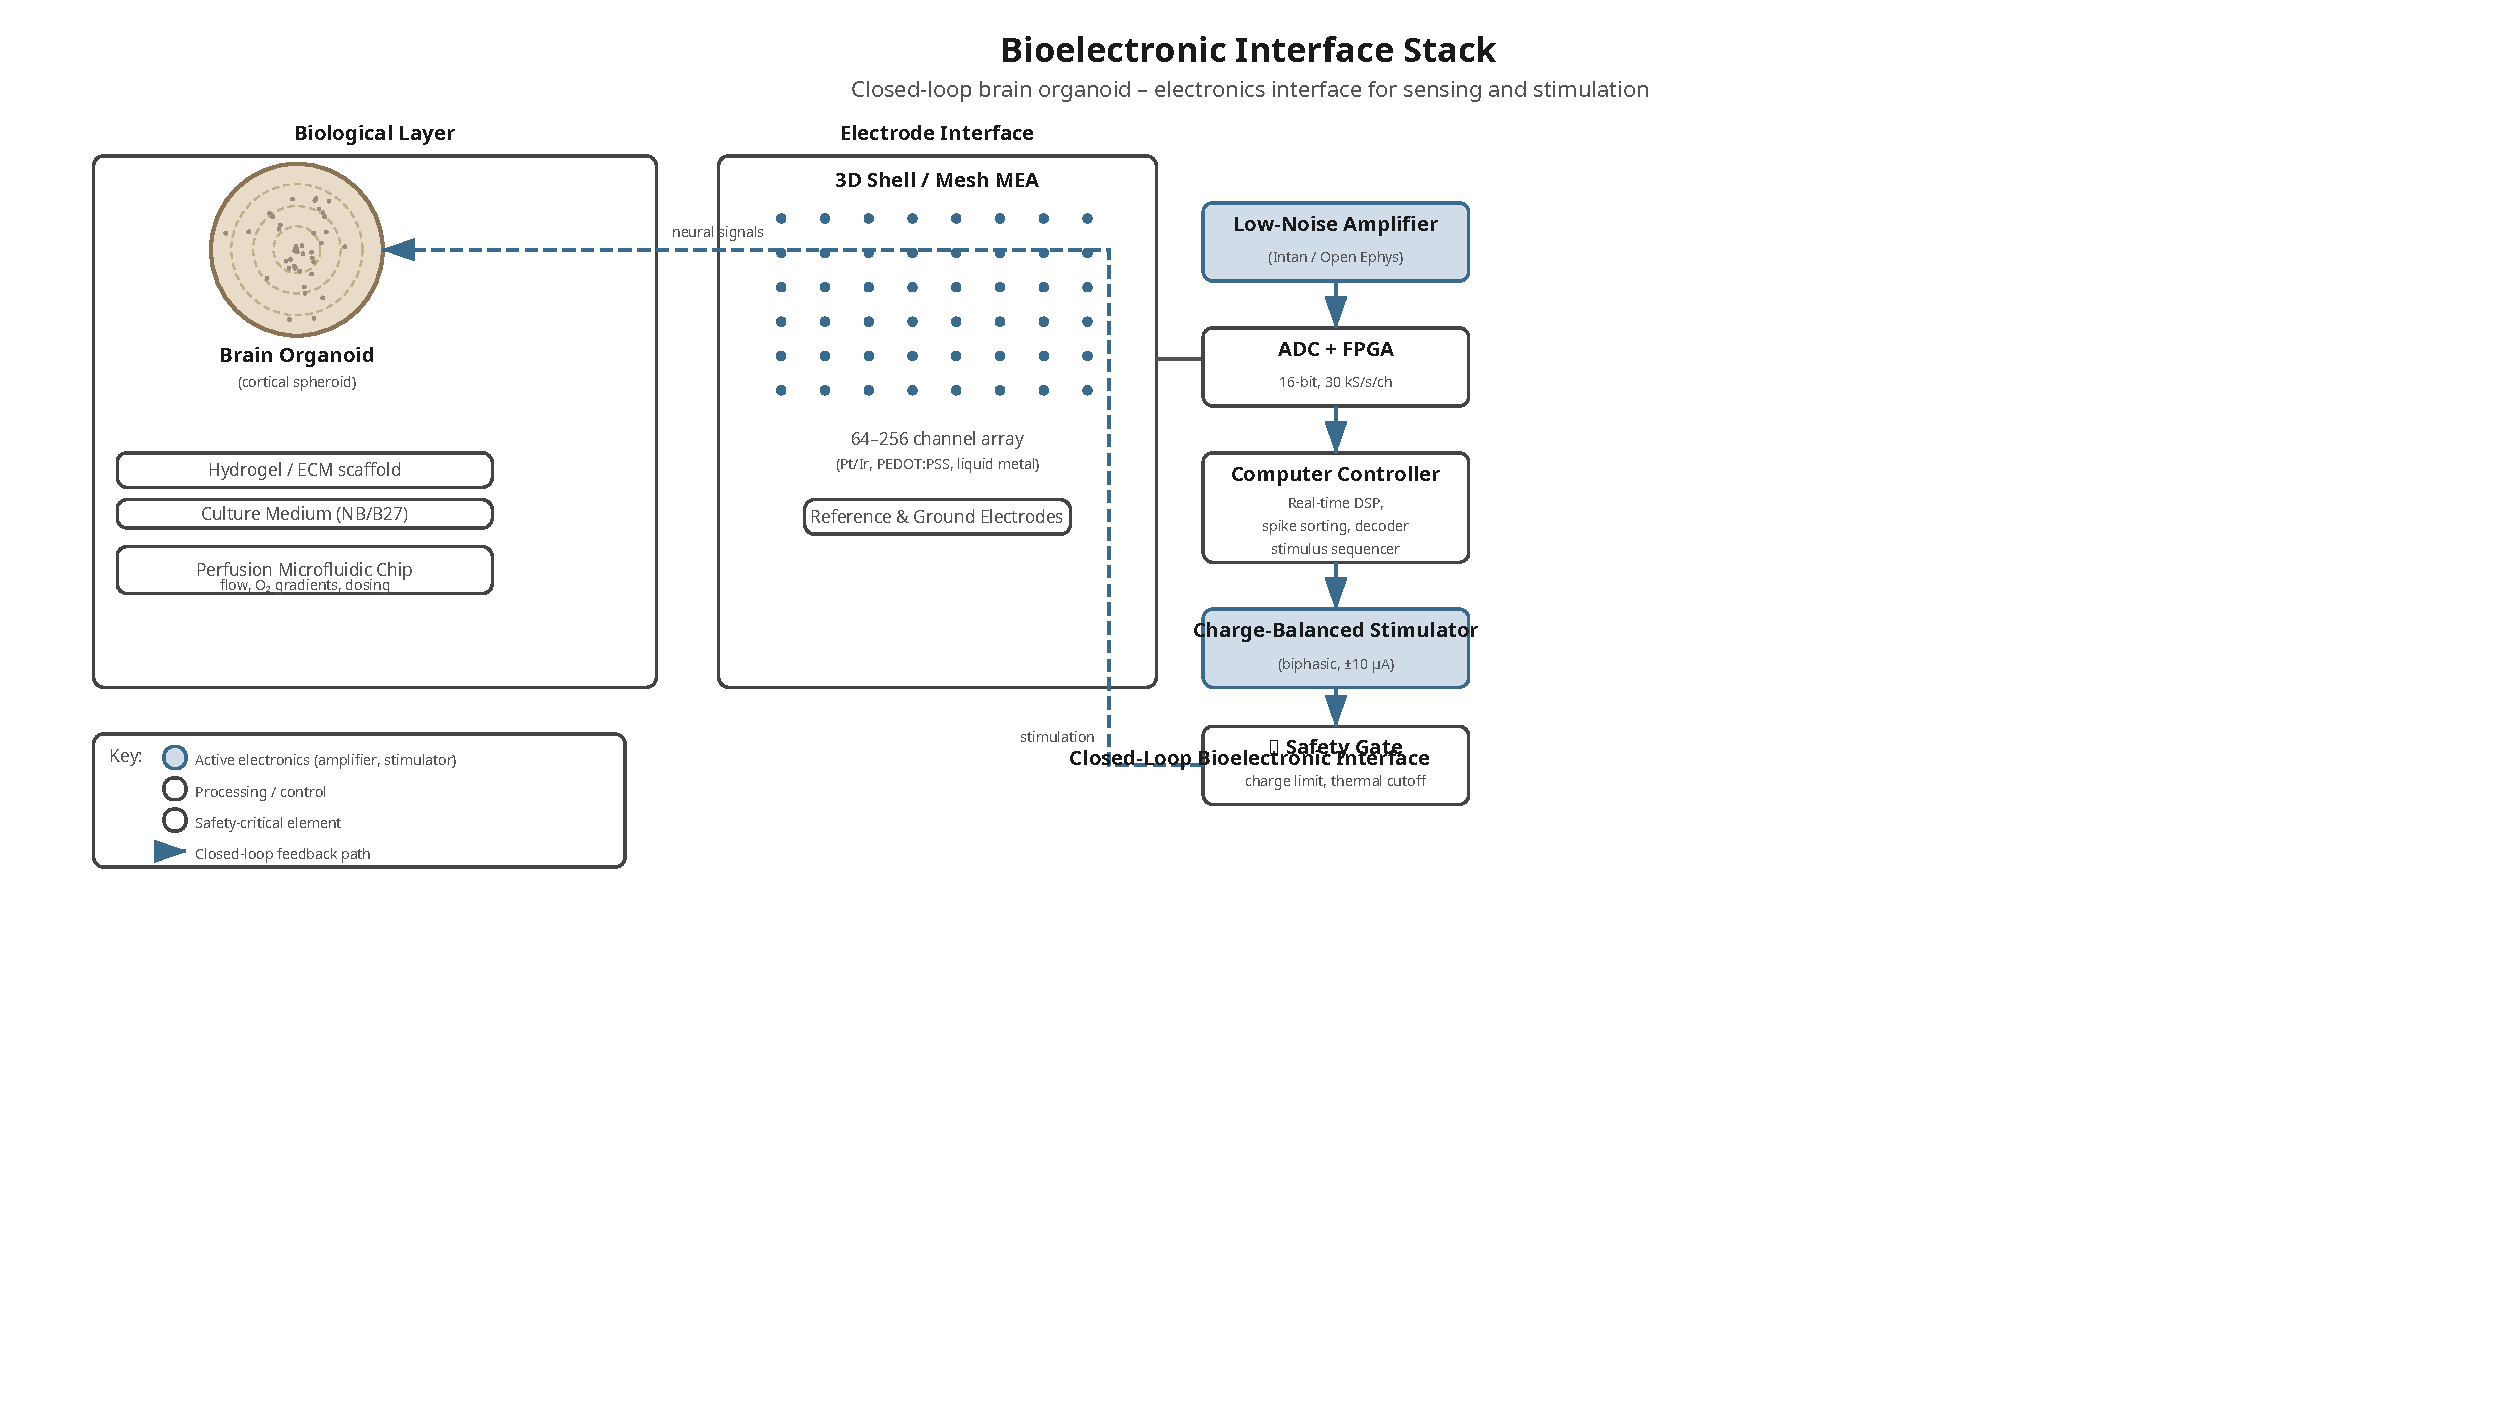
\includegraphics[width=\textwidth]{figures/biology_electronics_interface.pdf}
\caption{Feasible bioelectronic stack. The cell culture is never ``plugged into'' a computer directly. The electronics observe extracellular voltage, and the controller writes back through safe stimulation pulses.}
\end{figure*}

\begin{table*}[t]
\small
\caption{Build decisions that reduce the gap between biology and electronics.}
\begin{tabularx}{\textwidth}{p{0.18\textwidth}p{0.30\textwidth}X}
\toprule
\textbf{Layer} & \textbf{Practical choice} & \textbf{Why it makes the project feasible} \\
\midrule
Biology & Start with public data, a simulator, or a remote platform before local organoids & Removes cell-culture risk while validating the computational loop. \\
Recording & Use planar MEA data first; move to shell, mesh or 3D MEA only after analysis works & Planar MEA is simpler and has mature tools; 3D electrodes solve coverage later. \\
Stimulation & Use biphasic, charge-balanced pulses and strict software limits & Reduces electrode damage, electrochemistry and biological stress risk. \\
Signal path & Separate recording, stimulation, artifact blanking and feature extraction & Prevents the first demo from confusing stimulation artifact with biological response. \\
Control & Begin with rule-based burst feedback, then add reservoir/readout models & Gives an interpretable baseline before machine-learning claims. \\
Safety & Log every pulse, amplitude, duration, channel, tissue state and result & Makes the experiment auditable and easier to reproduce. \\
\bottomrule
\end{tabularx}
\end{table*}

\section{First Demo}

The first demo should be software-only and biologically honest: no organoid culture, no custom chip fabrication, and no claim of learning. The aim is to prove that the repository can run the complete control loop on realistic spike data. Use MEA-NAP-style channel spike times \cite{meanap2024}, FinalSpark-style remote notebooks when access exists \cite{finalspark_platform,finalspark2024}, or the Cortical Labs SDK/API examples for local development of closed-loop applications \cite{cl_api_doc,cl_sdk}. Closed-loop stimulation reviews emphasize that the controller must be faster than the biological process and that the chosen feature must be controllable \cite{tanskanen2020}.

\begin{figure*}[t]
\centering
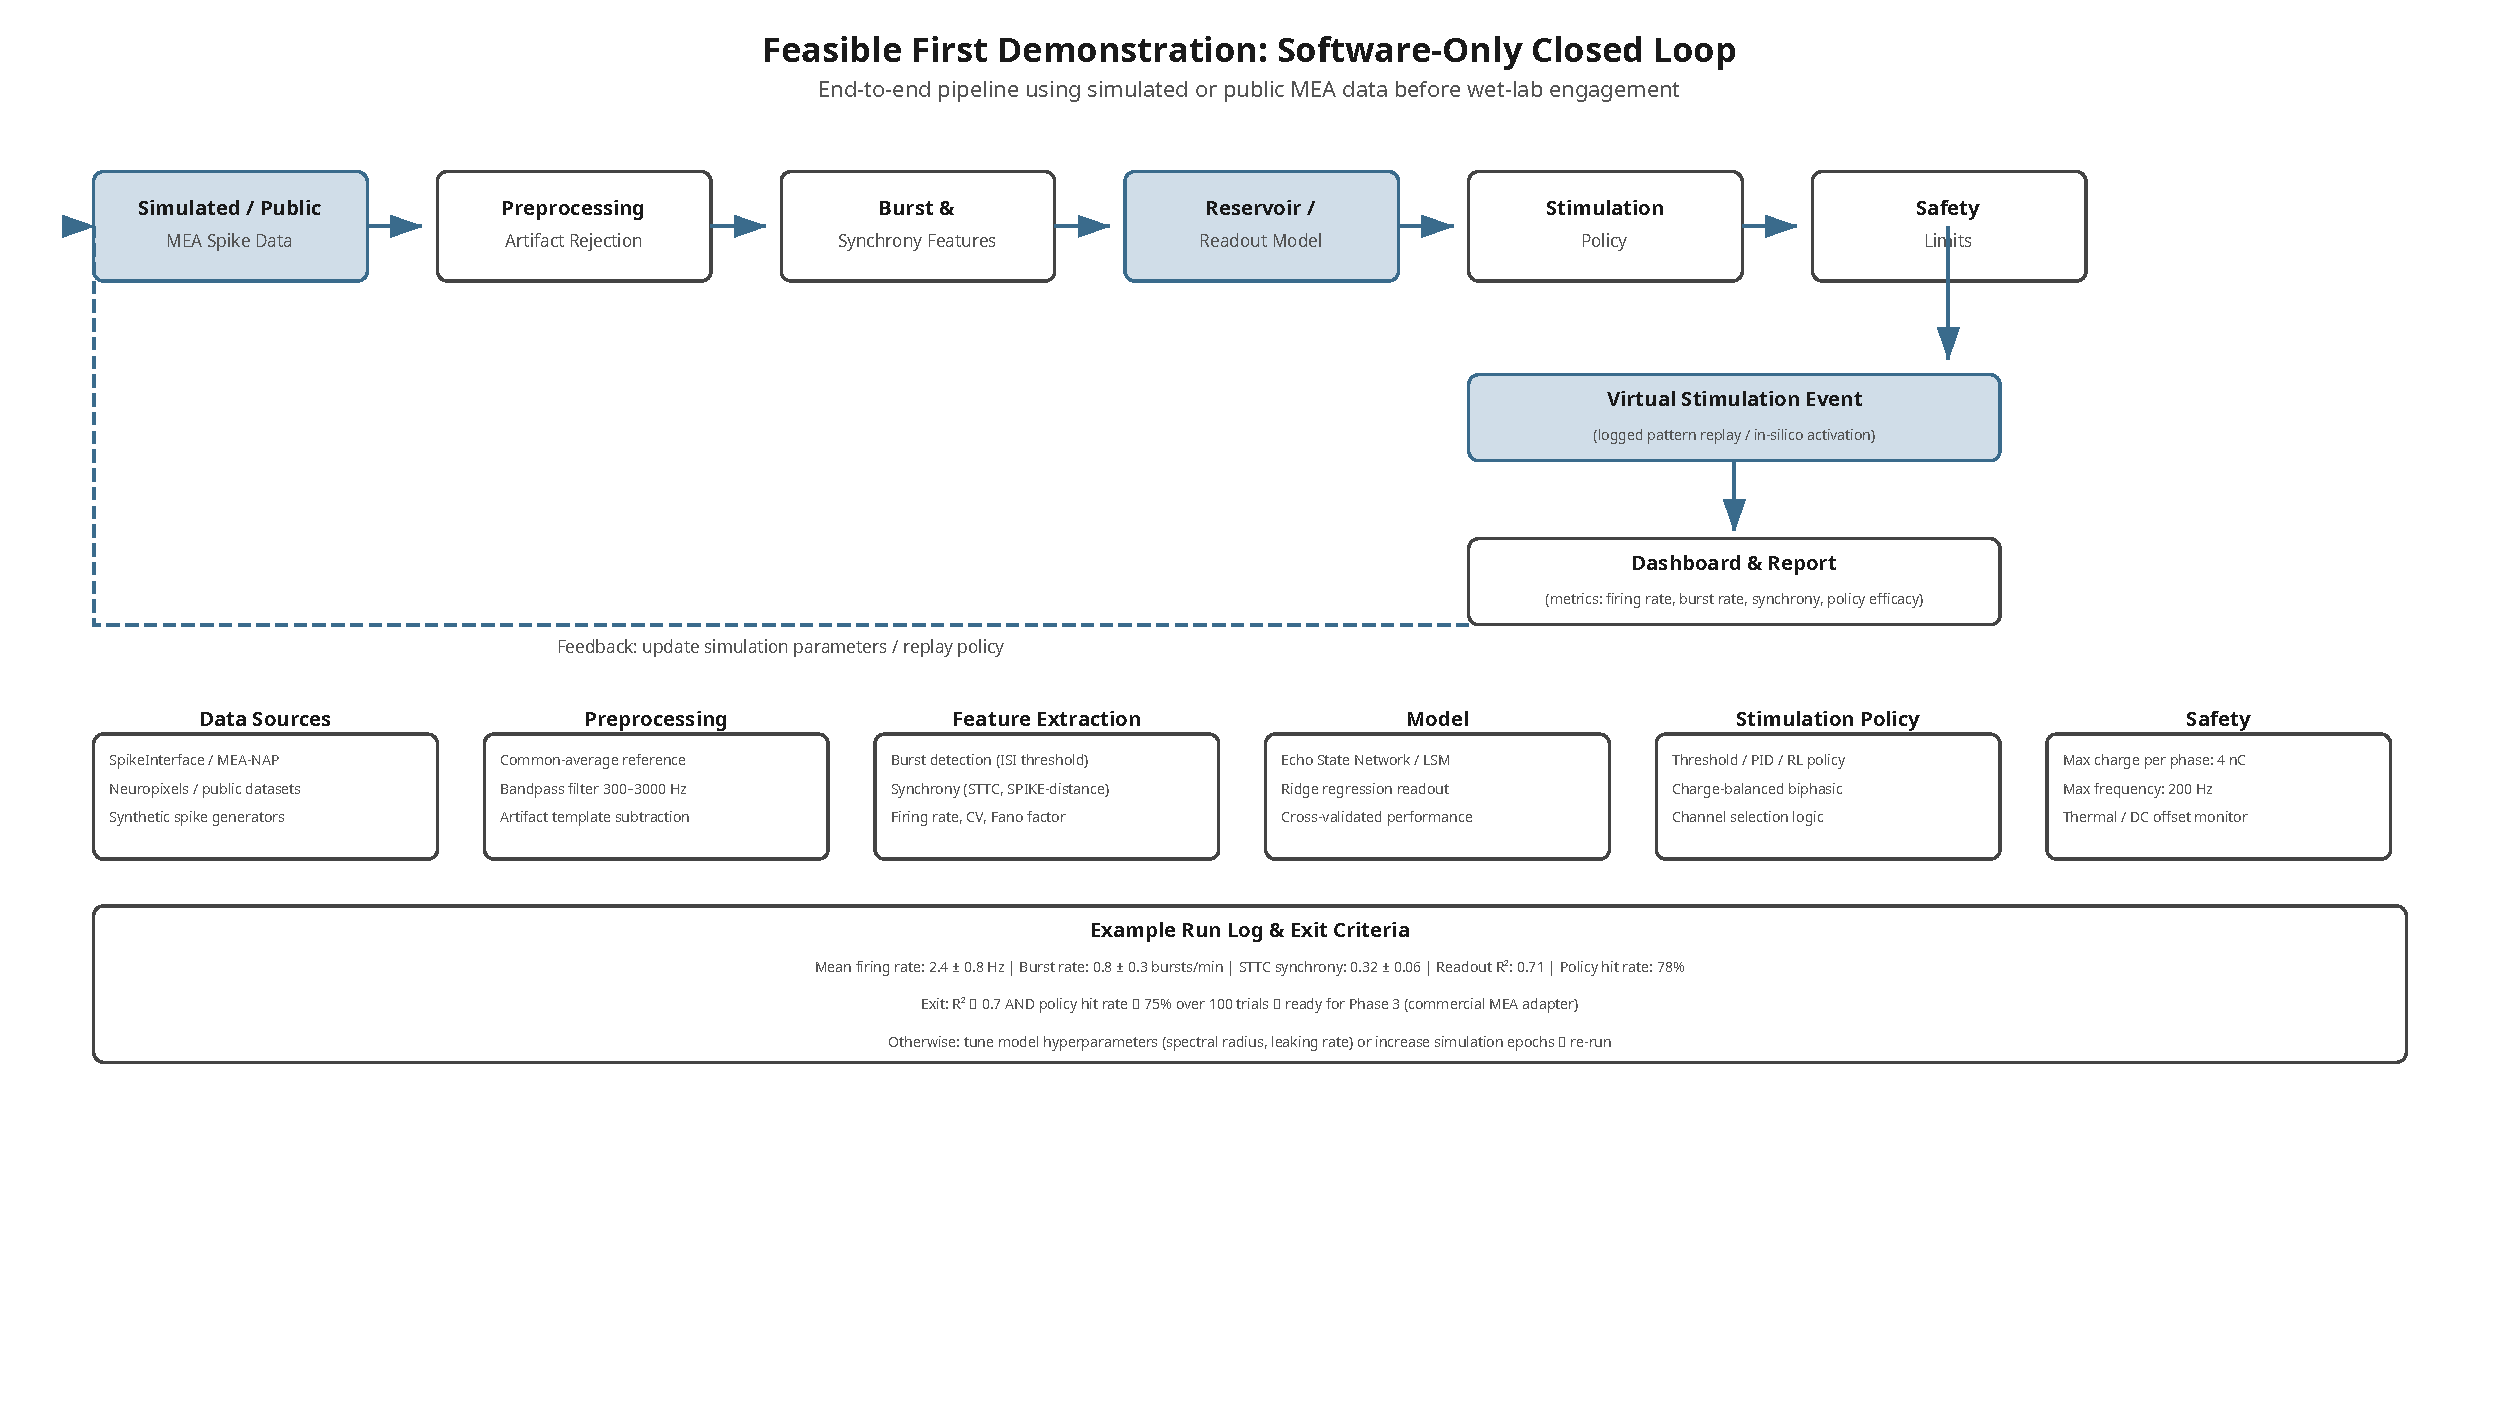
\includegraphics[width=\textwidth]{figures/first_demo_loop.pdf}
\caption{Minimum viable demo. It proves the digital side of the wetware loop before any living tissue is introduced.}
\end{figure*}

\textbf{Demo acceptance criteria.} A run should produce a single report with: input dataset hash or simulator seed, channel map, detected bursts, selected stimulation events, safety-limit decisions, latency estimate, and plots. Passing means the loop is reproducible and explainable, not that the organoid has learned.

\begin{table*}[t]
\small
\caption{Concrete implementation plan for the first two weeks.}
\begin{tabularx}{\textwidth}{p{0.12\textwidth}p{0.25\textwidth}X}
\toprule
\textbf{Step} & \textbf{Deliverable} & \textbf{Implementation detail} \\
\midrule
Day 1--2 & Repository skeleton & Add \texttt{experiments/first-demo/}, \texttt{data/manifests/}, and a README describing simulator-first scope. \\
Day 3--4 & Spike simulator & Generate Poisson plus bursting spike trains across 32--64 channels with fixed random seeds. \\
Day 5--6 & Feature extractor & Bin spikes, detect bursts, compute firing rate, inter-burst interval and channel synchrony. \\
Day 7--8 & Closed-loop policy & Trigger a virtual stimulation event when burst rate crosses a threshold or when synchrony drops. \\
Day 9--10 & Safety manager & Reject events that violate refractory interval, maximum pulses per minute or channel blacklist. \\
Day 11--12 & Dashboard/report & Save PNG/PDF plots and a machine-readable JSON run log. \\
Day 13--14 & Optional real-data adapter & Add importer for MEA-NAP-style outputs, FinalSpark notebook exports or Cortical Labs SDK streams. \\
\bottomrule
\end{tabularx}
\end{table*}

\section{Roadmap to Wet Biology}

\begin{figure*}[t]
\centering
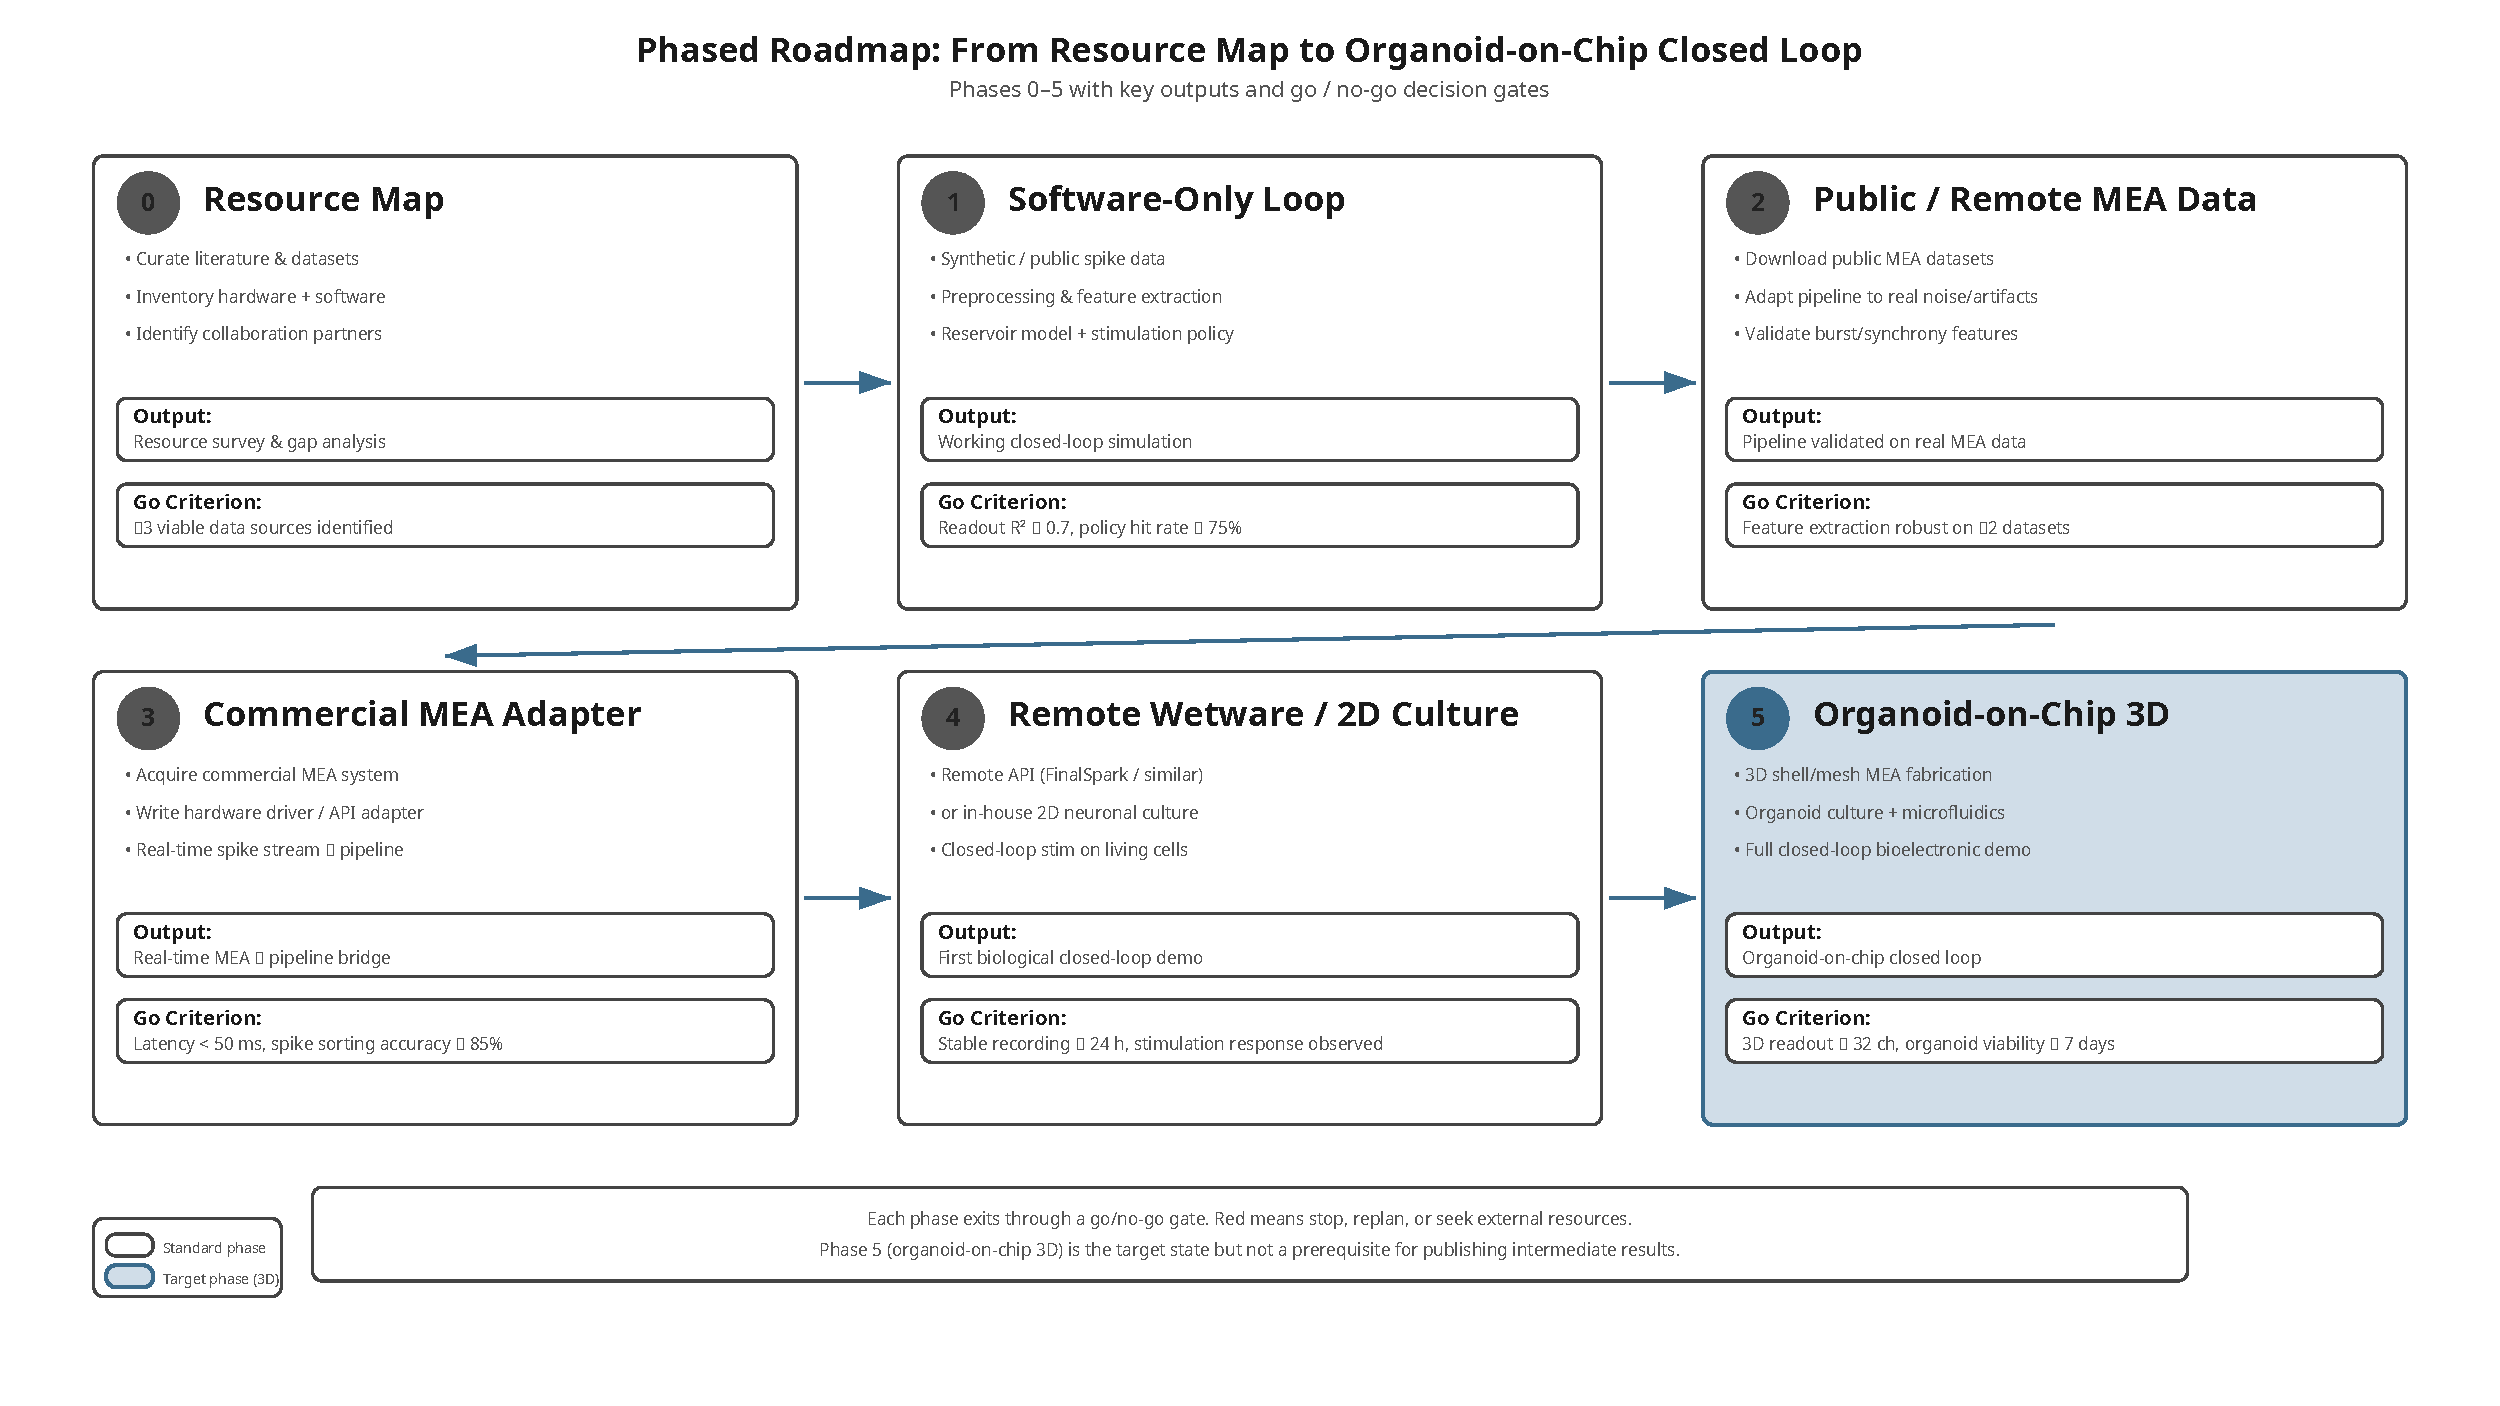
\includegraphics[width=\textwidth]{figures/phased_roadmap.pdf}
\caption{Phased roadmap. Each phase keeps the previous phase's software and replaces only one layer: simulator, data adapter, hardware adapter, then living tissue.}
\end{figure*}

The path becomes manageable if each phase has one new uncertainty. Phase 1 tests algorithms. Phase 2 tests real data. Phase 3 tests vendor APIs. Phase 4 tests living neural tissue without custom fabrication. Phase 5 tests custom organoid geometry and 3D interfaces. This sequence follows the direction of emerging bioelectronics reviews: start with MEA-compatible measurements, then improve geometric coupling and chronic stability \cite{bioelectronics2022}.

\section{Research Gaps}

The next useful project should not start by claiming general intelligence. It should build a reproducible loop: standardized organoid culture, 3D MEA geometry, stimulation protocol, common data format, analysis notebook, and ethics log. The most publishable near-term experiments are comparative: planar MEA versus shell/mesh/3D MEA; static culture versus perfused culture; open-loop stimulation versus adaptive closed-loop stimulation; single-organoid versus organoid-array ensembles.

\section{Recommended Repository Direction}

For this repository, the most valuable structure is:
\begin{itemize}
\item \texttt{references/papers/}: PDFs and citation metadata.
\item \texttt{references/repos/}: vendored snapshots or submodules for code references.
\item \texttt{publications/}: this survey and later manuscripts.
\item \texttt{experiments/}: future notebooks for MEA signal analysis, reservoir computing, and closed-loop simulations.
\item \texttt{data/}: only small public example datasets; keep large electrophysiology data external with manifest files.
\end{itemize}

\section{Companion Repository}

OrganoidVision is the companion repository for retinal-organoid sensing and bio-hybrid vision systems \cite{organoidvision2026}. OrganoidIntelligence should remain the broad roadmap for brain-on-chip intelligence, while OrganoidVision develops the application branch for organoid sensors, optical stimulation, event-based vision and sensor-stack blueprints.

\section{Conclusion}

Brain-organoid-on-chip systems are best understood as engineered interfaces around living neural tissue. The field's practical center is disease modelling, toxicology and electrophysiology. Organoid intelligence adds a computing agenda, but its credibility depends on careful controls, repeatable closed-loop protocols, and open analysis. The strongest resource path for this repository is to combine curated papers, reproducible MEA tools, and explicit project tracking for FinalSpark, Cortical Labs, NSF BEGIN OI, and open organoid data efforts.

\begin{thebibliography}{99}\small

\bibitem{lancaster2013} Lancaster, M. A. et al. Cerebral organoids model human brain development and microcephaly. \emph{Nature} 501, 373--379 (2013). \url{https://pubmed.ncbi.nlm.nih.gov/23995685/}
\bibitem{karzbrun2018} Karzbrun, E. et al. Human brain organoids on a chip reveal the physics of folding. \emph{Nature Physics} 14, 515--522 (2018). \url{https://pubmed.ncbi.nlm.nih.gov/29760764/}
\bibitem{wang2018} Wang, Y., Wang, L., Zhu, Y. \& Qin, J. Human brain organoid-on-a-chip to model prenatal nicotine exposure. \emph{Lab on a Chip} 18, 851--860 (2018). \url{https://doi.org/10.1039/C7LC01084B}
\bibitem{ao2020} Ao, Z. et al. One-stop microfluidic assembly of human brain organoids to model prenatal cannabis exposure. \emph{Analytical Chemistry} 92, 4630--4638 (2020). \url{https://doi.org/10.1021/acs.analchem.0c00205}
\bibitem{cho2021} Cho, A.-N. et al. Microfluidic device with brain extracellular matrix promotes structural and functional maturation of human brain organoids. \emph{Nature Communications} 12, 4730 (2021). \url{https://www.nature.com/articles/s41467-021-24775-5}
\bibitem{ao2021} Ao, Z. et al. Tubular human brain organoids to model microglia-mediated neuroinflammation. \emph{Lab on a Chip} 21, 2751--2762 (2021). \url{https://doi.org/10.1039/D1LC00030F}
\bibitem{castiglione2022} Castiglione, H. et al. Human brain organoids-on-chip: advances, challenges, and perspectives for preclinical applications. \emph{Pharmaceutics} 14, 2301 (2022). \url{https://pmc.ncbi.nlm.nih.gov/articles/PMC9699341/}
\bibitem{zhang2025} Zhang, H. et al. Brain organoids-on-chip for neural diseases modeling: history, challenges and trends. \emph{Journal of Pharmaceutical Analysis} 15, 101323 (2025). \url{https://pubmed.ncbi.nlm.nih.gov/41208919/}
\bibitem{zhao2024} Zhao, Y. et al. Integrating organoids and organ-on-a-chip devices. \emph{Nature Reviews Bioengineering} 2, 588--608 (2024). \url{https://www.nature.com/articles/s44222-024-00207-z}
\bibitem{meanap2024} MEA-NAP: a flexible network analysis pipeline for neuronal 2D and 3D organoid multielectrode recordings. \url{https://pmc.ncbi.nlm.nih.gov/articles/PMC11706071/}
\bibitem{hdmea2022} Functional imaging of brain organoids using high-density microelectrode arrays. \url{https://pmc.ncbi.nlm.nih.gov/articles/PMC9474390/}
\bibitem{park2021} Park, Y. et al. Three-dimensional, multifunctional neural interfaces for cortical spheroids and engineered assembloids. \emph{Science Advances} 7, eabf9153 (2021). \url{https://pmc.ncbi.nlm.nih.gov/articles/PMC7968849/}
\bibitem{li2019} Li, Q. et al. Cyborg organoids: implantation of nanoelectronics via organogenesis for tissue-wide electrophysiology. \emph{Nano Letters} 19, 5781--5789 (2019). \url{https://pubmed.ncbi.nlm.nih.gov/31347851/}
\bibitem{lefloch2022} Le Floch, P. et al. Stretchable mesh nanoelectronics for three-dimensional single-cell chronic electrophysiology from developing brain organoids. \emph{Advanced Materials} 34, 2106829 (2022). \url{https://pmc.ncbi.nlm.nih.gov/articles/PMC8930507/}
\bibitem{huang2022} Huang, Q. et al. Shell microelectrode arrays (MEAs) for brain organoids. \emph{Science Advances} 8, eabq5031 (2022). \url{https://pubmed.ncbi.nlm.nih.gov/35977026/}
\bibitem{wu2024} Wu, Y. et al. Three-dimensional liquid metal-based neuro-interfaces for human hippocampal organoids. \emph{Nature Communications} 15, 4047 (2024). \url{https://www.nature.com/articles/s41467-024-48452-5}
\bibitem{magnetic2025} Magnetically reshapable 3D multi-electrode arrays of liquid metals for electrophysiological analysis of brain organoids. \url{https://pmc.ncbi.nlm.nih.gov/articles/PMC11868496/}
\bibitem{kim2026} Kim, N. et al. Multilayered microelectrode array for monitoring electrophysiological signals of 3d neural networks in cerebral organoid. \emph{Microsystems \& Nanoengineering} 12, 201 (2026). \url{https://www.nature.com/articles/s41378-026-01328-8}
\bibitem{shapeconformal2026} Liu, N. et al. Shape-conformal porous frameworks for full coverage of neural organoids and high-resolution electrophysiology. \emph{Nature Biomedical Engineering} (2026). \url{https://www.nature.com/articles/s41551-026-01620-y}
\bibitem{bioelectronics2022} Tasnim, K. \& Liu, J. Emerging bioelectronics for brain organoid electrophysiology. \emph{Journal of Molecular Biology} 434, 167165 (2022). \url{https://pmc.ncbi.nlm.nih.gov/articles/PMC8766612/}
\bibitem{tanskanen2020} Tanskanen, J. M. A., Ahtiainen, A. \& Hyttinen, J. A. K. Toward closed-loop electrical stimulation of neuronal systems: a review. \emph{Bioelectricity} 2, 328--347 (2020). \url{https://pmc.ncbi.nlm.nih.gov/articles/PMC8370352/}
\bibitem{smirnova2023} Smirnova, L. et al. Organoid intelligence (OI): the new frontier in biocomputing and intelligence-in-a-dish. \emph{Frontiers in Science} 1, 1017235 (2023). \url{https://www.frontiersin.org/articles/10.3389/fsci.2023.1017235/full}
\bibitem{baltimore2023} Hartung, T. et al. The Baltimore Declaration toward the exploration of organoid intelligence. \emph{Frontiers in Science} 1, 1068159 (2023). \url{https://doi.org/10.3389/fsci.2023.1068159}
\bibitem{workshop2023} Morales Pantoja, I. E. et al. First Organoid Intelligence (OI) workshop to form an OI community. \emph{Frontiers in Artificial Intelligence} 6, 1116870 (2023). \url{https://par.nsf.gov/biblio/10484679-first-organoid-intelligence-oi-workshop-form-oi-community}
\bibitem{cai2023} Cai, H. et al. Brain organoid reservoir computing for artificial intelligence. \emph{Nature Electronics} 6, 1032--1039 (2023). \url{https://www.nature.com/articles/s41928-023-01069-w}
\bibitem{kagan2022} Kagan, B. J. et al. In vitro neurons learn and exhibit sentience when embodied in a simulated game-world. \emph{Neuron} 110, 3952--3969.e8 (2022). \url{https://pubmed.ncbi.nlm.nih.gov/36228614/}
\bibitem{khajehnejad2024} Khajehnejad, M. et al. Biological neurons compete with deep reinforcement learning in sample efficiency in a simulated gameworld. arXiv:2405.16946 (2024). \url{https://arxiv.org/abs/2405.16946}
\bibitem{finalspark2024} Jordan, F. et al. Open and remotely accessible Neuroplatform for research in wetware computing. \emph{Frontiers in Artificial Intelligence} (2024). \url{https://pmc.ncbi.nlm.nih.gov/articles/PMC11097343/}
\bibitem{talavera2025} Talavera, Y. \& Ulmann, B. Brain organoid computing: an overview. arXiv:2503.19770 (2025). \url{https://arxiv.org/abs/2503.19770}
\bibitem{liu2025} Liu, T., Philamore, H. \& Ward-Cherrier, B. Encoding tactile stimuli for Braille recognition with organoids. arXiv:2508.20850 (2025/2026). \url{https://arxiv.org/abs/2508.20850}
\bibitem{finalspark_platform} FinalSpark Neuroplatform. \url{https://finalspark.com/neuroplatform/}
\bibitem{cortical_platform} Cortical Labs CL1 and Cortical Cloud. \url{https://corticallabs.com/}
\bibitem{cl_api_doc} Cortical Labs CL API Documentation Pre-Release. \url{https://github.com/Cortical-Labs/cl-api-doc}
\bibitem{cl_sdk} Cortical Labs CL SDK. \url{https://github.com/Cortical-Labs/cl-sdk}
\bibitem{cl_spikestream} Cortical Labs SpikeStream visualisation code. \url{https://github.com/Cortical-Labs/SpikeStream}
\bibitem{openorganoid} OpenOrganoid. \url{https://openorganoid.org/}
\bibitem{nsf_begin_oi} NSF EFRI BEGIN OI program materials. \url{https://www.nsf.gov/funding/opportunities/emerging-frontiers-research-innovation-efri-biocomputing/13708/updates/96870}
\bibitem{axion} Axion BioSystems Organoid MEA. \url{https://files.axionbiosystems.com/products/mea-plates/organoid-mea}
\bibitem{mcs_mesh} Harvard Bioscience / Multi Channel Systems Mesh MEA. \url{https://www.harvardbioscience.com/products/organoid-electrophysiology}
\bibitem{netri} NETRI NeuroFluidics MEA. \url{https://netri.com/netri-launches-neurofluidics-mea-new-line/}
\bibitem{mimetas} MIMETAS OrganoPlate. \url{https://www.mimetas.com/}
\bibitem{organoidvision2026} Chen, L. \& AgintiFlow. Bio-Hybrid Vision Systems: Engineering Retinal Organoids as Advanced Imaging Sensors. OrganoidVision repository (2026). \url{https://github.com/lachlanchen/organoid-vision}

\end{thebibliography}

\end{document}
